\documentclass[a4paper,twocolumn]{article}
\usepackage[hmargin={1.1cm,1.1cm},vmargin={2.2cm,2cm}]{geometry}
%       includehead,     scale=0.85,centering,hoffset=-0.1cm,voffset=-0.5cm]{geometry} headheight=13.1pt ,portrait

%\usepackage[a4paper,portrait,twocolumn,includeheadfoot,
%            scale=0.85,centering,hoffset=-1cm]{geometry}
\usepackage[pdftex]{graphicx,color}
\usepackage{amsmath}
\usepackage{amssymb}
\usepackage{stmaryrd}
\usepackage[french]{babel}
\selectlanguage{french}
\usepackage{fancyhdr}
\usepackage{floatflt}
\usepackage{ucs}
\usepackage[utf8]{inputenc}
\usepackage[T1]{fontenc}
\usepackage[pdftex,colorlinks={true},urlcolor={blue},pdfauthor={remy Nicolai}]{hyperref}
\usepackage{makeidx}


%Options de hyperref pour les fichiers pdf g{\'e}n{\'e}r{\'e}s
%\hypersetup{pdfpagemode=None,colorlinks=true,pdffitwindow=true}
%\hypersetup{pdfpagemode=None,colorlinks=true}


%                 Chargement des symboles de l'AMS
%\input amssym
%pour que la compilation aille au bout
%\nofiles\scrollmode

%pr{\'e}sentation du compteur de niveau 2 dans les listes
\makeatletter
\renewcommand{\labelenumii}{\theenumii.}
\makeatother

%dimension des pages, en-t{\^e}te et bas de page
  %utilisation avec vmargin
   %\setpapersize{custom}{21cm}{29.7cm}
   %\setmarginsrb{1.5cm}{0cm}{3.5cm}{1cm}{15mm}{10mm}{0mm}{0mm}
%\setlength{\voffset}{-2cm}
%\setlength{\oddsidemargin}{-1cm}
%\setlength{\textheight}{25cm}
%\setlength{\textwidth}{17.3cm}
%\columnsep=5pt
% \columnseprule=0.5pt
%\columnseprule=0.5pt
%En tete et pied de page
\pagestyle{fancy}
\lhead{Lycée Hoche MPSI B}
%\rhead{}
%\rhead{25/11/05}
\lfoot{\tiny{Cette création est mise à disposition selon le Contrat\\ Paternité-Partage des Conditions Initiales à l'Identique 2.0 France\\ disponible en ligne http://creativecommons.org/licenses/by-sa/2.0/fr/
} }
\rfoot{\tiny{Rémy Nicolai \jobname pdf du \today}}

%\pagestyle{fancy}
%\lhead{MPSI B}
%\rhead{\today}
%\rfoot{\small{\jobname}}
\newcommand{\baseurl}{http://back.maquisdoc.net/data/}
\newcommand{\textesurl}{http://back.maquisdoc.net/data/devoirs_nicolair/}
\newcommand{\exosurl}{http://back.maquisdoc.net/data/exos_nicolair/}
\newcommand{\coursurl}{http://back.maquisdoc.net/data/cours_nicolair/}

\newcommand{\N}{\mathbb{N}}
\newcommand{\Z}{\mathbb{Z}}
\newcommand{\C}{\mathbb{C}}
\newcommand{\R}{\mathbb{R}}
\newcommand{\K}{\mathbf{K}}
\newcommand{\Q}{\mathbb{Q}}
\newcommand{\F}{\mathbf{F}}
\newcommand{\U}{\mathbb{U}}
\newcommand{\p}{\mathbb{P}}


\newcommand{\card}{\mathop{\mathrm{Card}}}
\newcommand{\Id}{\mathop{\mathrm{Id}}}
\newcommand{\Ker}{\mathop{\mathrm{Ker}}}
\newcommand{\Vect}{\mathop{\mathrm{Vect}}}
\newcommand{\cotg}{\mathop{\mathrm{cotan}}}
\newcommand{\cotan}{\mathop{\mathrm{cotan}}}
\newcommand{\sh}{\mathop{\mathrm{sh}}}
\newcommand{\ch}{\mathop{\mathrm{ch}}}
\newcommand{\argch}{\mathop{\mathrm{argch}}}
\newcommand{\argsh}{\mathop{\mathrm{argsh}}}
\newcommand{\tr}{\mathop{\mathrm{tr}}}
\newcommand{\rg}{\mathop{\mathrm{rg}}}
\newcommand{\rang}{\mathop{\mathrm{rg}}}
\newcommand{\val}{\mathop{\mathrm{val}}}

\newcommand{\Mat}{\mathop{\mathrm{Mat}}}
\newcommand{\MatB}[2]{\mathop{\mathrm{Mat}}_{\mathcal{#1}}\left( #2\right) }
\newcommand{\MatBB}[3]{\mathop{\mathrm{Mat}}_{\mathcal{#1} \mathcal{#2}}\left( #3\right) }

\renewcommand{\Re}{\mathop{\mathrm{Re}}}
\newcommand{\Ima}{\mathop{\mathrm{Im}}}
\renewcommand{\Im}{\mathop{\mathrm{Im}}}
\renewcommand{\th}{\mathop{\mathrm{th}}}
\newcommand{\repere}{$(O,\overrightarrow{i},\overrightarrow{j},\overrightarrow{k})$ }
\newcommand{\trans}{\mathstrut^t\!}
\newcommand{\cov}{\mathop{\mathrm{Cov}}}
\newcommand{\orth}[1]{#1^{\perp}}

\newcommand{\absolue}[1]{\left| #1 \right|}
\newcommand{\fonc}[5]{#1 : \begin{cases}#2 &\rightarrow #3 \\ #4 &\mapsto #5 \end{cases}}
\newcommand{\depar}[2]{\dfrac{\partial #1}{\partial #2}}
\newcommand{\norme}[1]{\left\| #1 \right\|}
\newcommand{\se}{\geq}
\newcommand{\ie}{\leq}
\newcommand{\serie}[1]{\left( \sum {#1}_n \right)_{n\in\N}}

\batchmode
 
\begin{document} 
\chead{ courbes paramétrées: énoncés.}
\begin{enumerate}
  \item \begin{tiny}(Ecr01)\end{tiny}
Pour les courbes suivantes, {\'e}tudier les points demand{\'e}s et reconnaitre le support parmi les figures proposées\\
% use packages: array
\renewcommand{\arraystretch}{3.6}
\begin{tabular}{|c|p{3.1cm}|p{3.8cm}|}\hline 
1 & $(\frac{2t}{t^{2}-1},\frac{(t+1)^{2}}{t^{2}})$ & points doubles, branches infinies. \\ \hline 
2 & $(\cos 3t,\sin 2t)$ & points multiples. \\ \hline
3 & $(t+\frac{1}{t},t^{2}+\frac{1}{t^{2}})$ & {\'e}quation cart{\'e}sienne. \\ \hline
4 & $(\frac{t^{3}}{(t-1)(t+2)},\frac{t(t-2)}{t-1})$ & branches infinies. \\ \hline
5 & $(te^{t},\frac{1}{t}e^{t})$ & branches infinies, points d'inflexion. \\ \hline
6 & $(t(1-e^{t}),\ln (\cosh t))$ & branches infinies, points stationnaires. \\ \hline
7 & $\begin{aligned}
(\frac{1}{t}+\frac{2}{t+1}+\frac{3}{t-1},\\
\frac{2}{t}+\frac{3}{t+1}+\frac{1}{t-1})  
 \end{aligned}$
 & branches infinies. \\ \hline
\end{tabular}
\begin{figure}[ht]
   \centering
   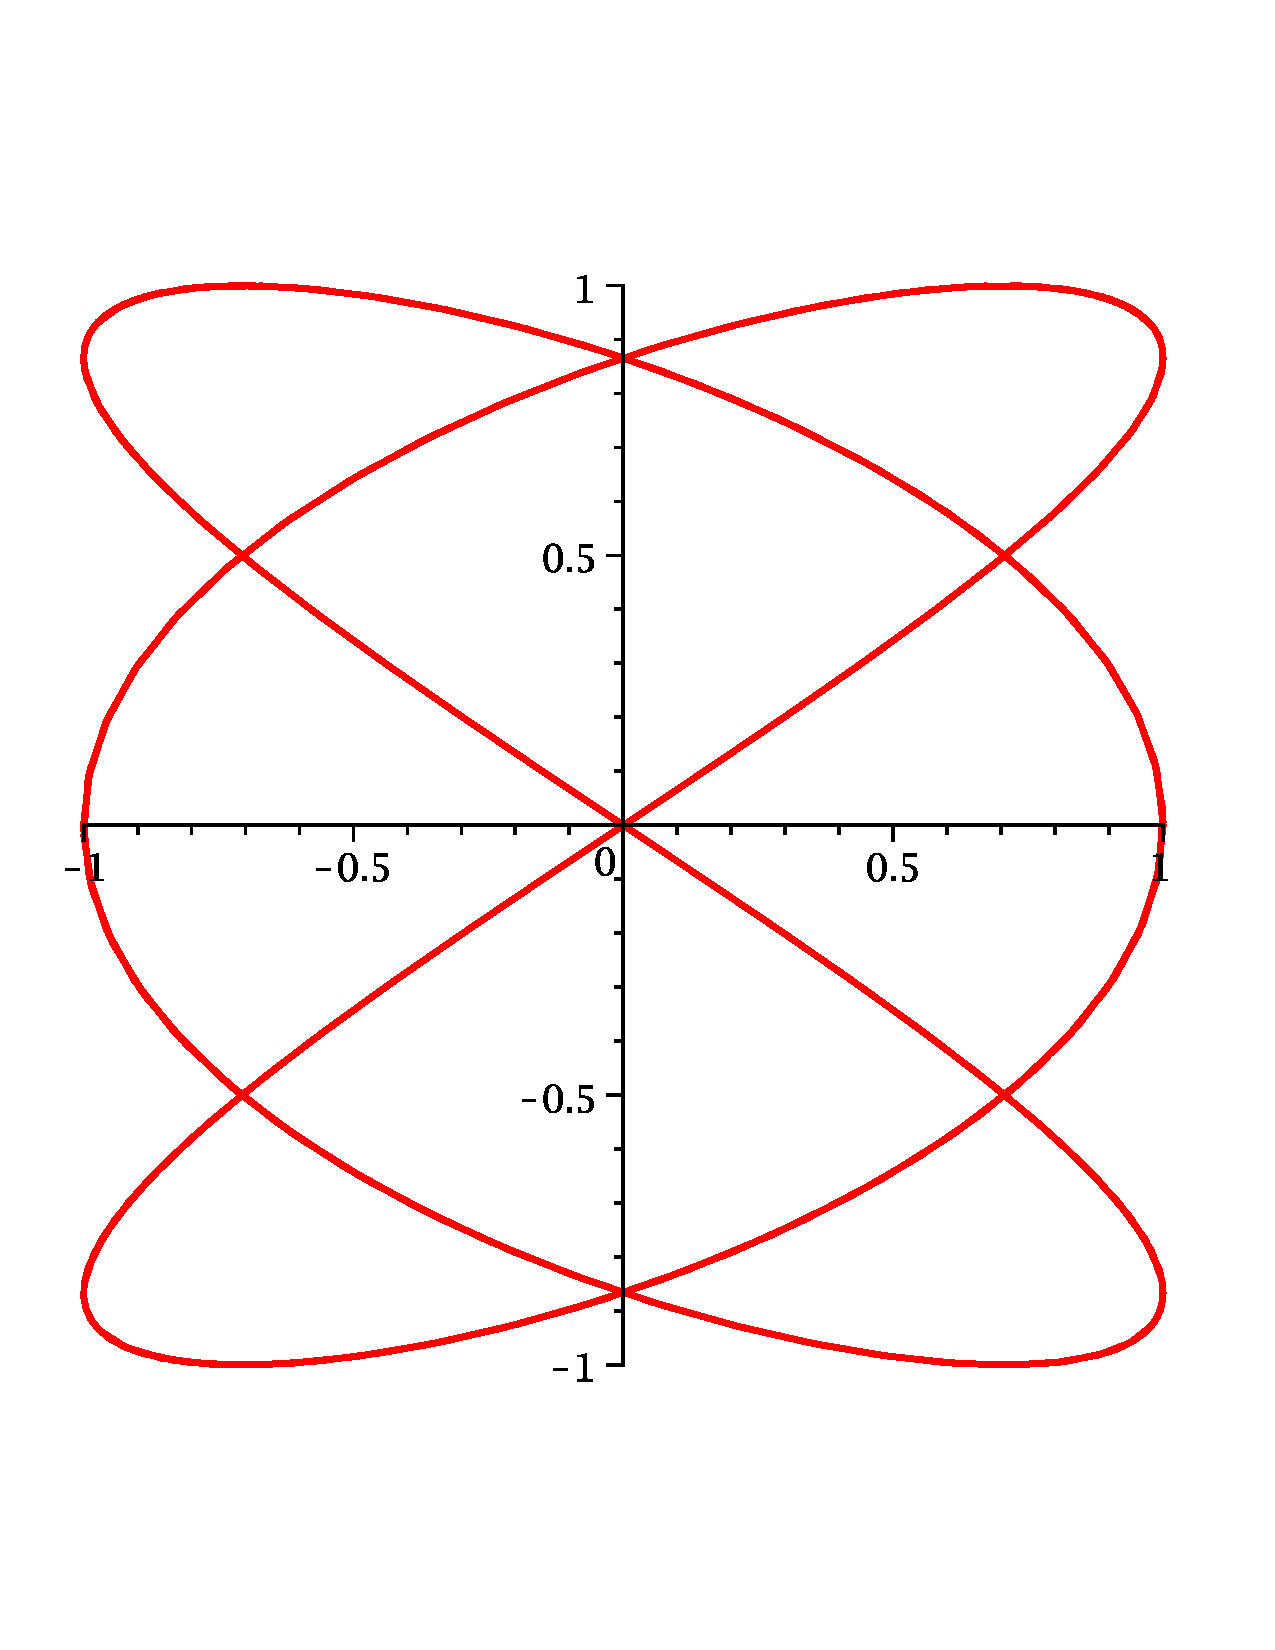
\includegraphics[width=5cm]{Ecr01_1.pdf}
   \caption{Exercice \arabic{enumi} : courbe 1}
\end{figure}
\begin{figure}[ht]
   \centering
   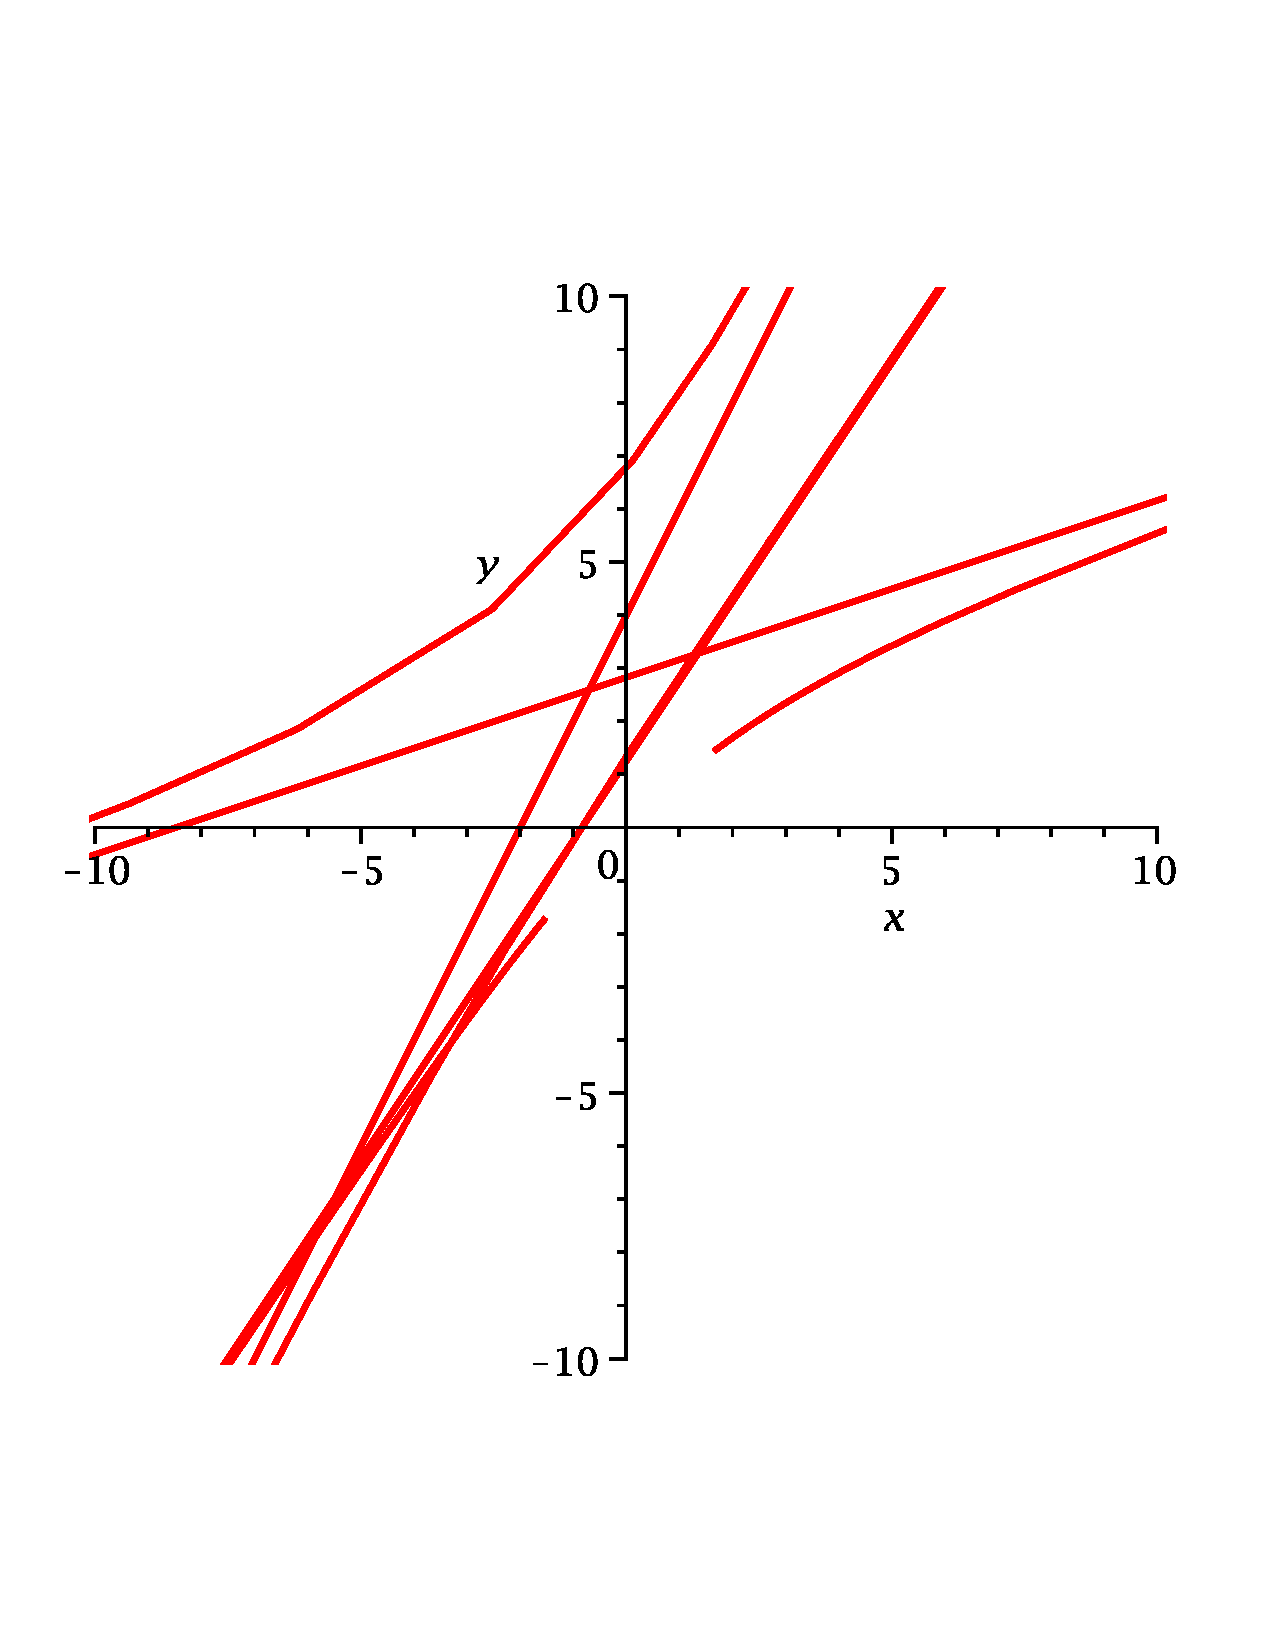
\includegraphics[width=5cm]{Ecr01_2.pdf}
   \caption{Exercice \arabic{enumi} : courbe 2}
\end{figure}
\begin{figure}[ht]
   \centering
   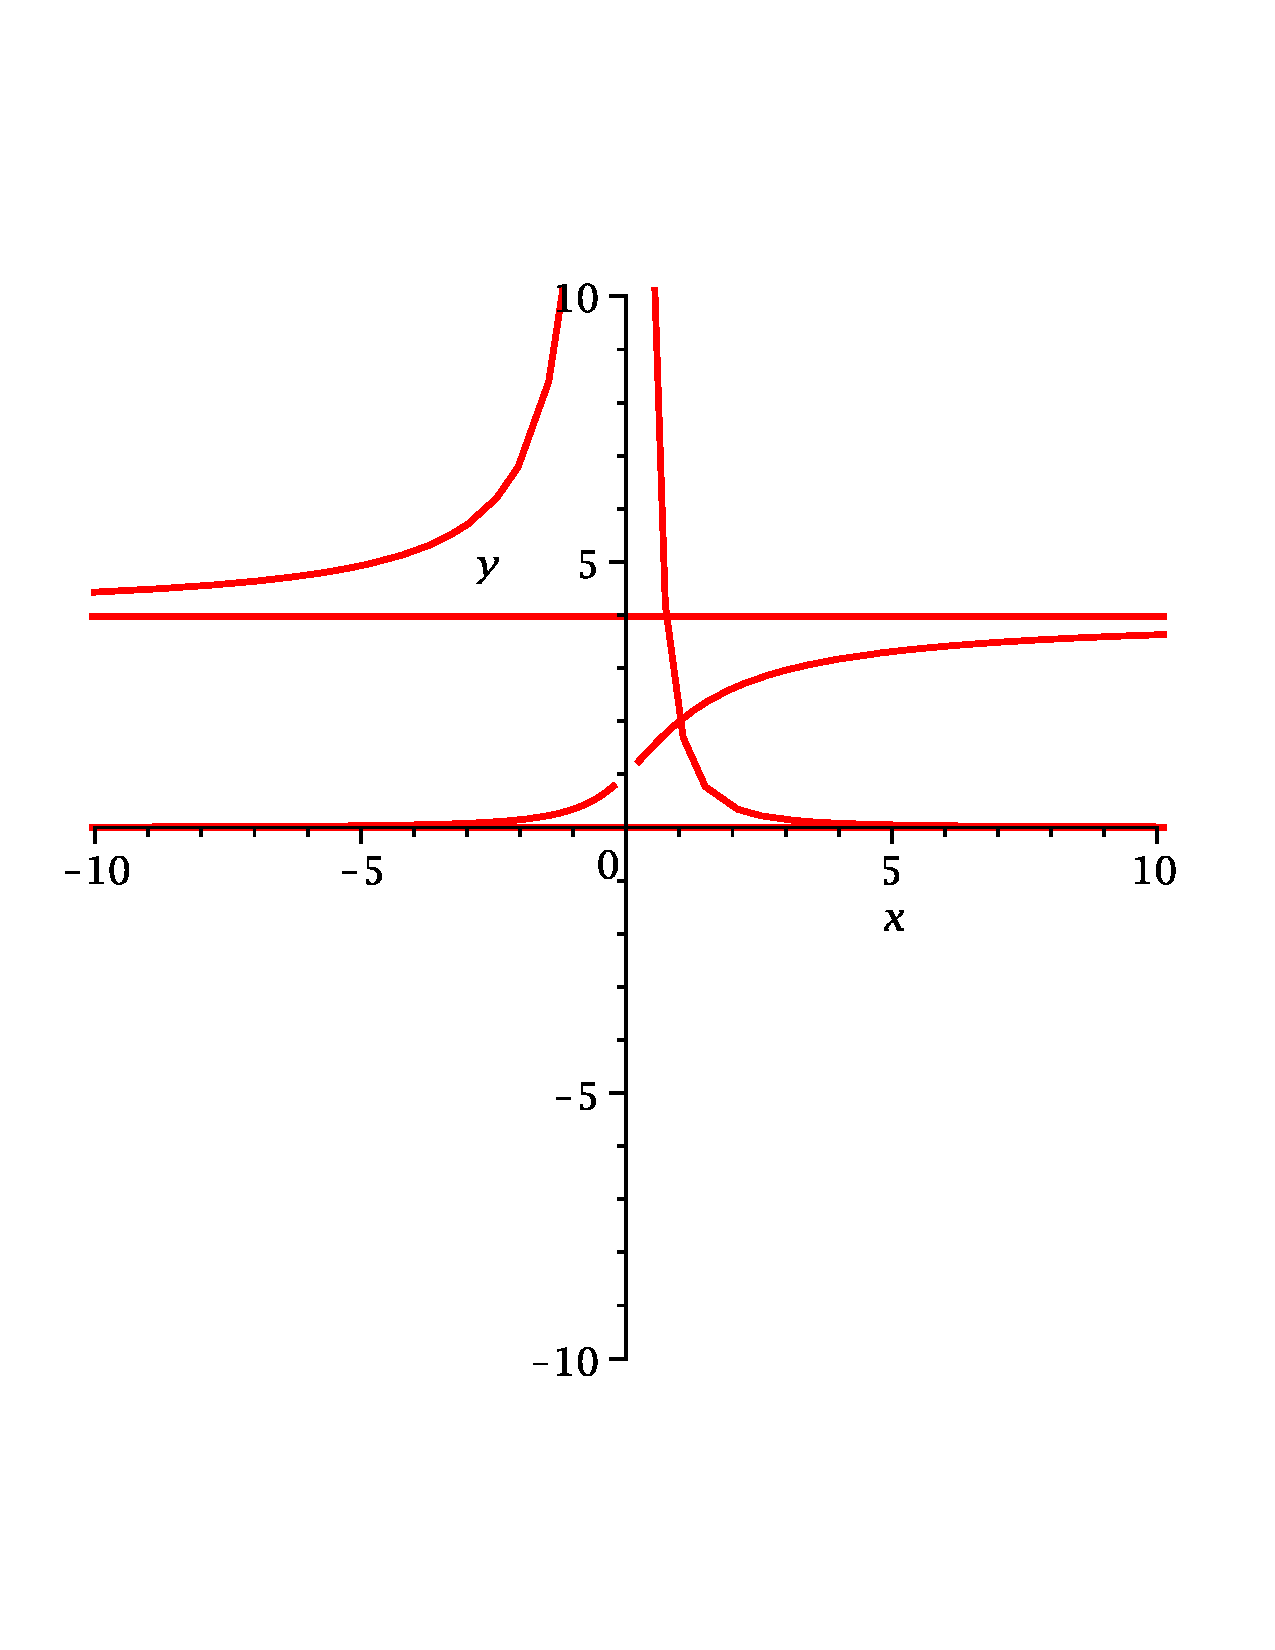
\includegraphics[scale=0.25]{Ecr01_3.pdf}
   \caption{Exercice \arabic{enumi} : courbe 3}
\end{figure}
\begin{figure}[ht]
   \centering
   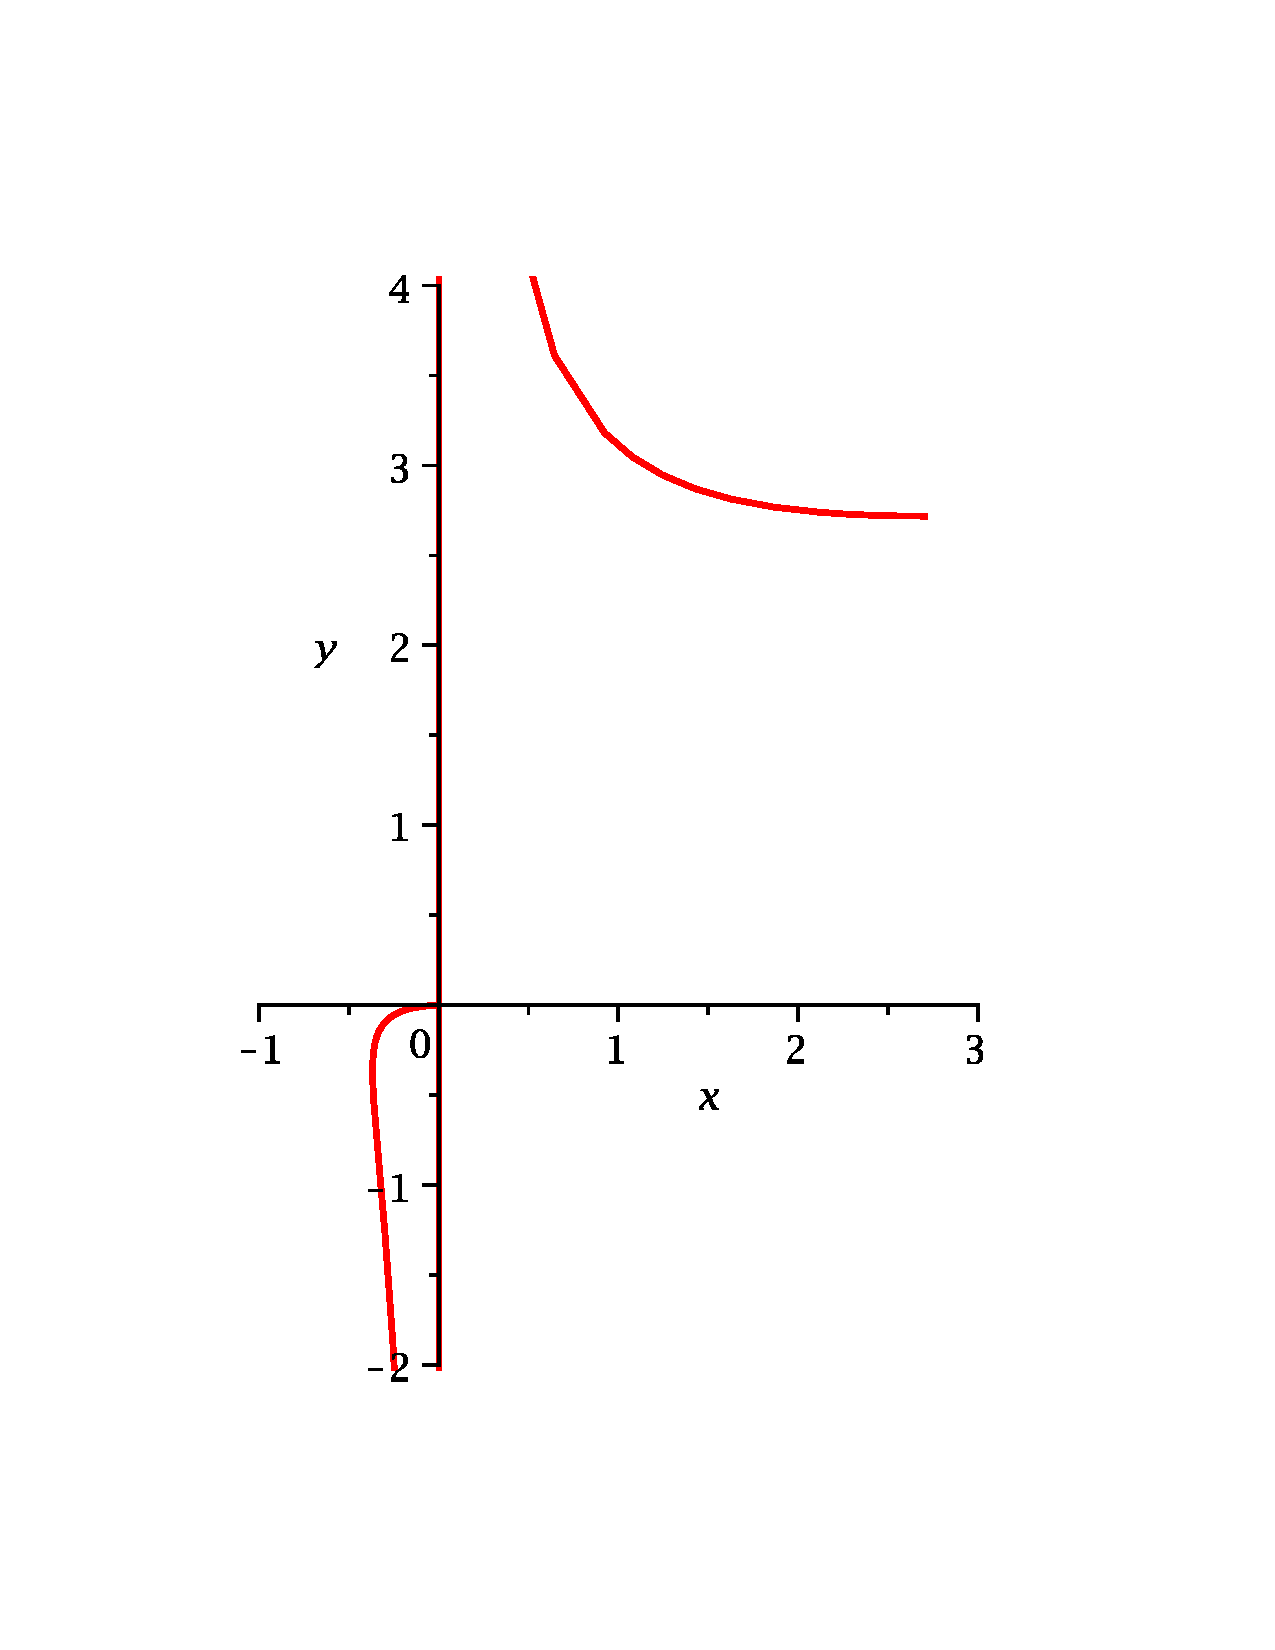
\includegraphics[scale=0.25]{Ecr01_4.pdf}
   \caption{Exercice \arabic{enumi} : courbe 4}
\end{figure}
\begin{figure}[ht]
   \centering
   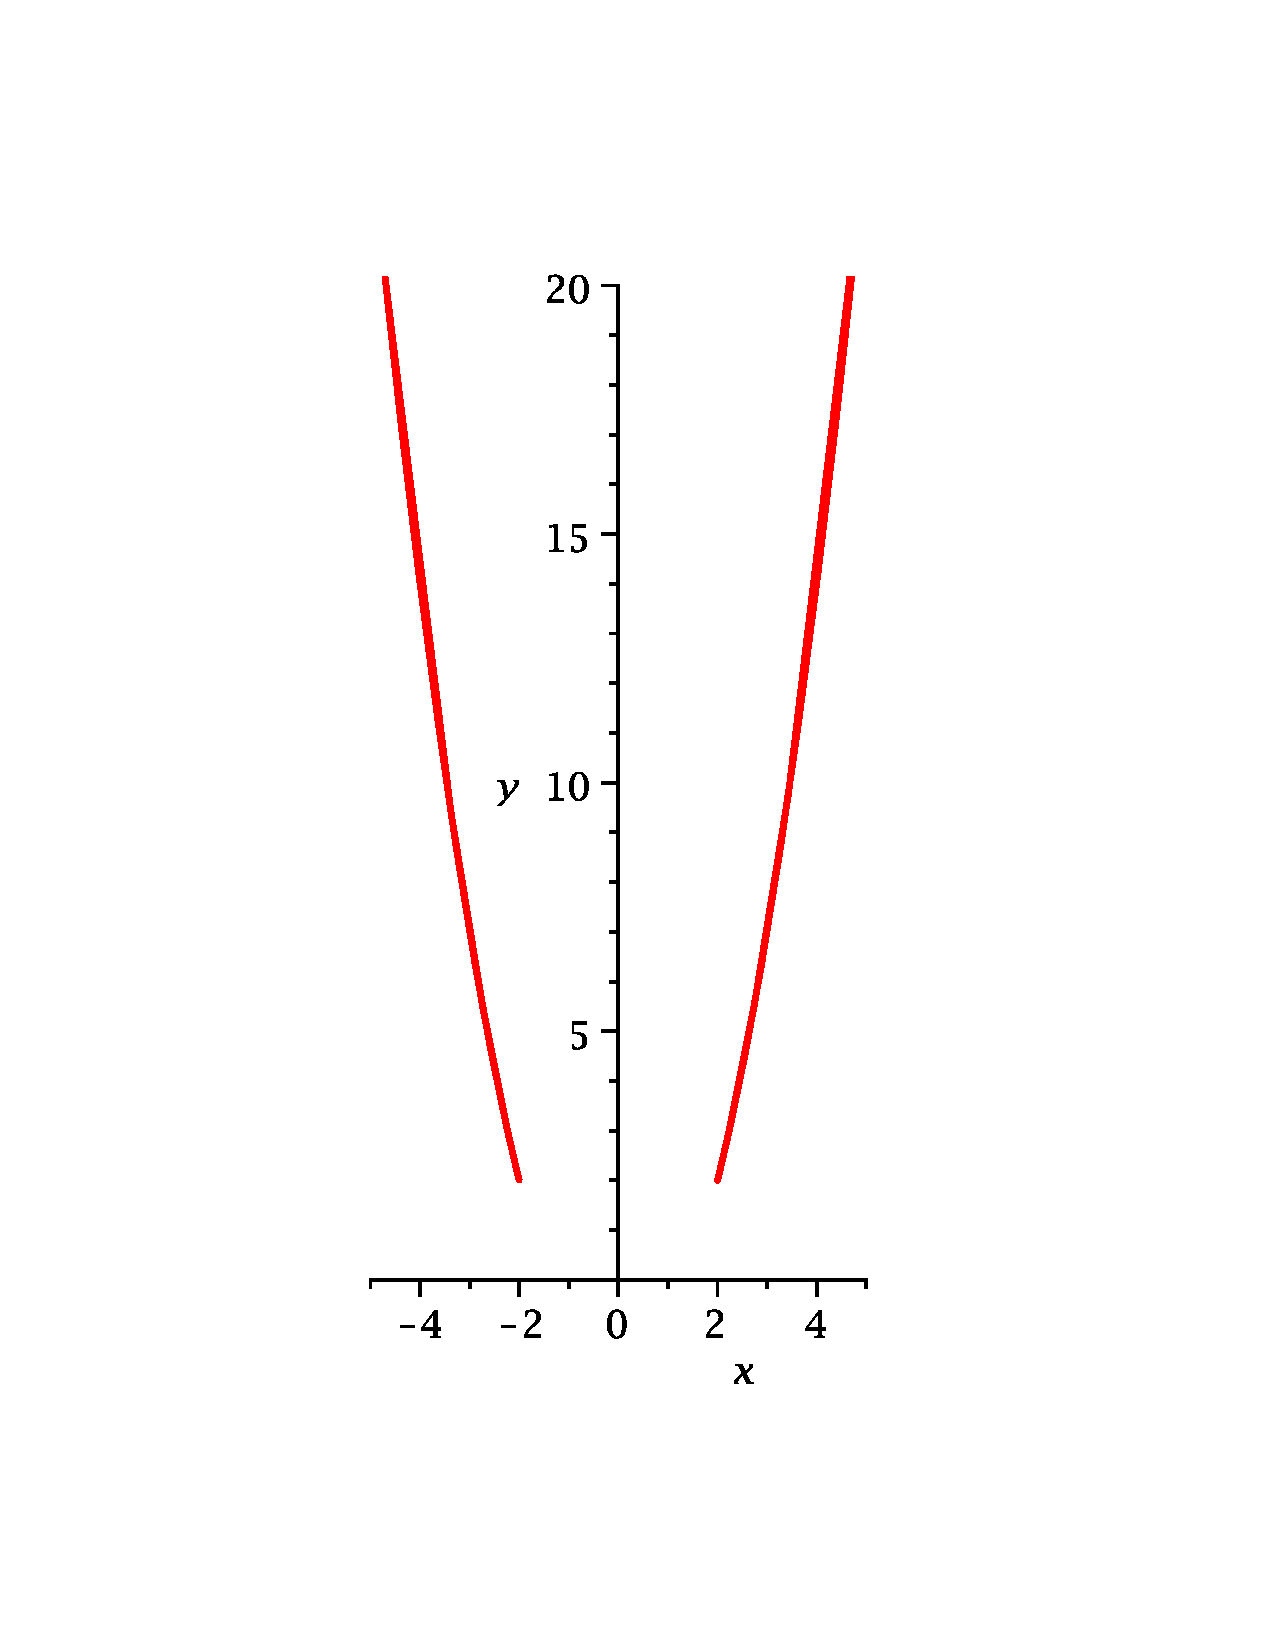
\includegraphics[scale=0.25]{Ecr01_5.pdf}
   \caption{Exercice \arabic{enumi} : courbe 5}
\end{figure}
\begin{figure}[ht]
   \centering
   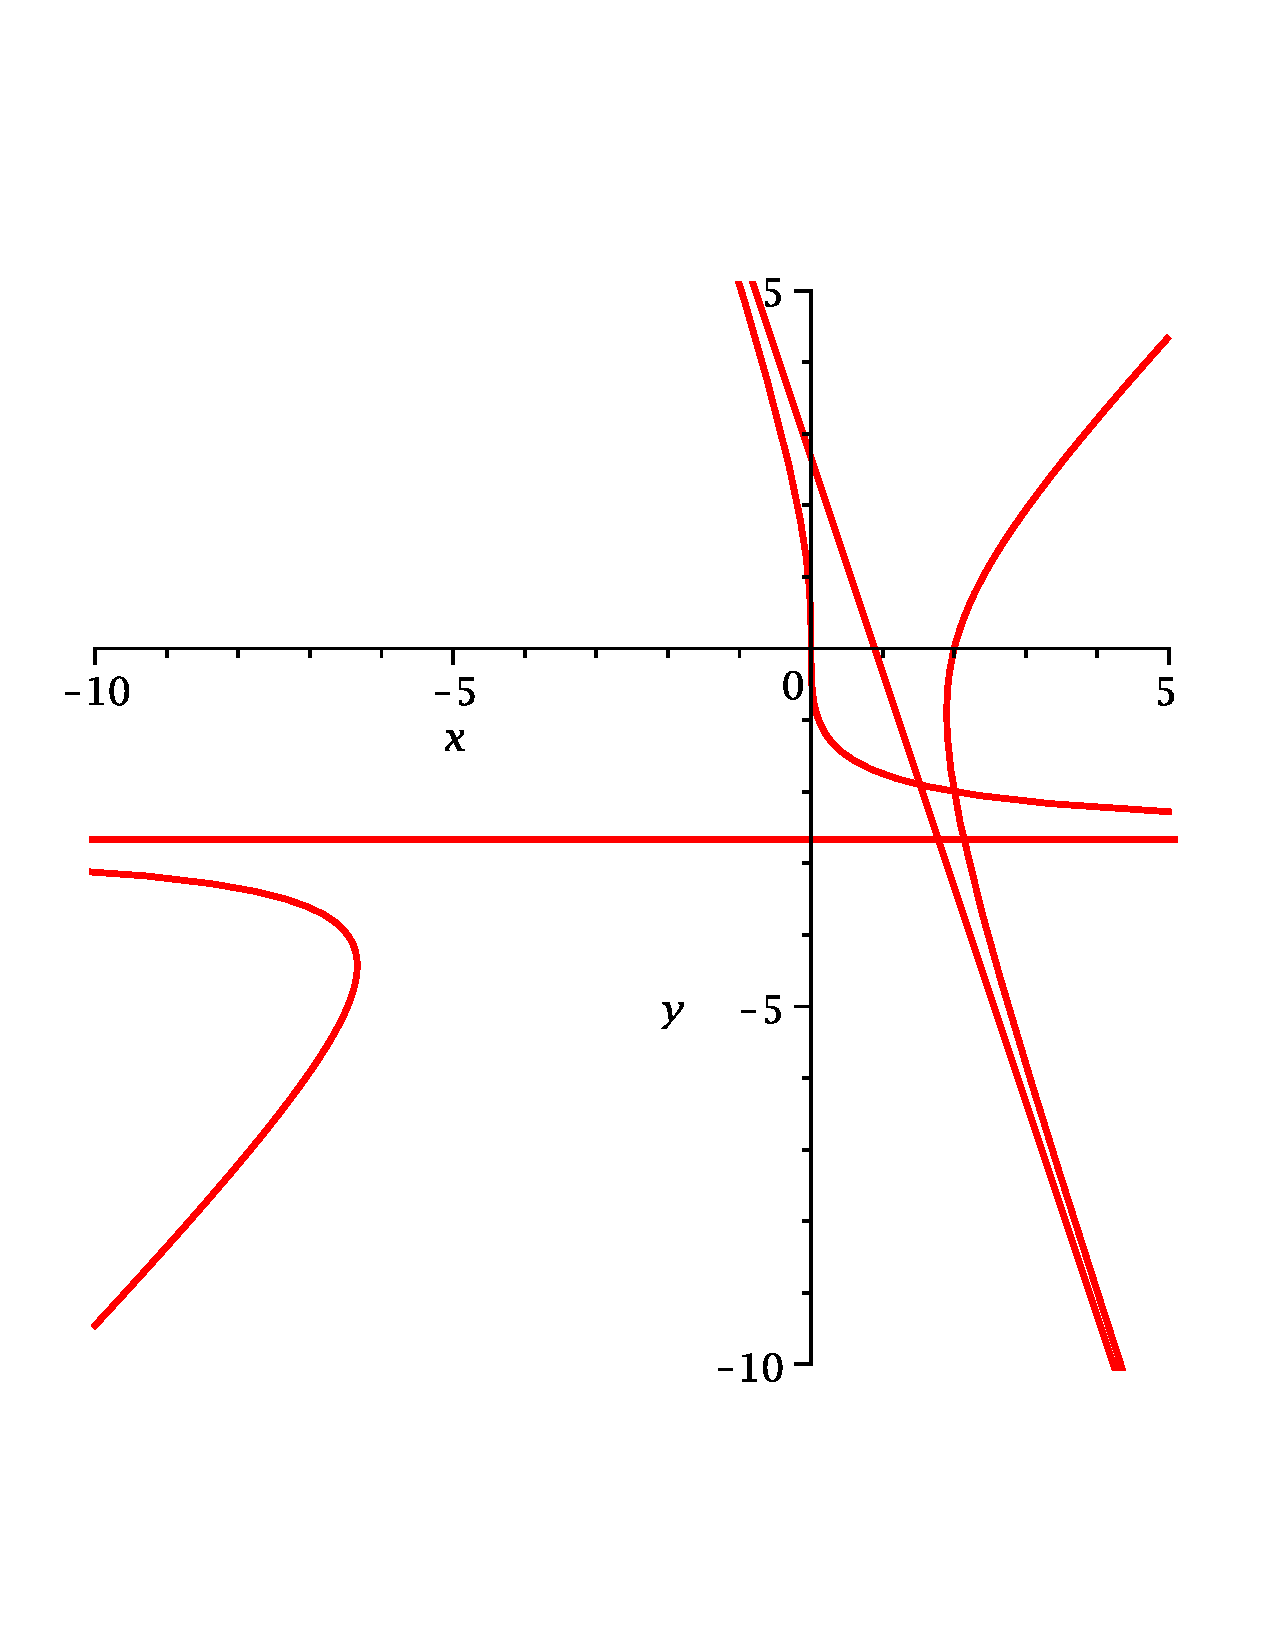
\includegraphics[scale=0.25]{Ecr01_6.pdf}
   \caption{Exercice \arabic{enumi} : courbe 6}
\end{figure}
\begin{figure}[ht]
   \centering
   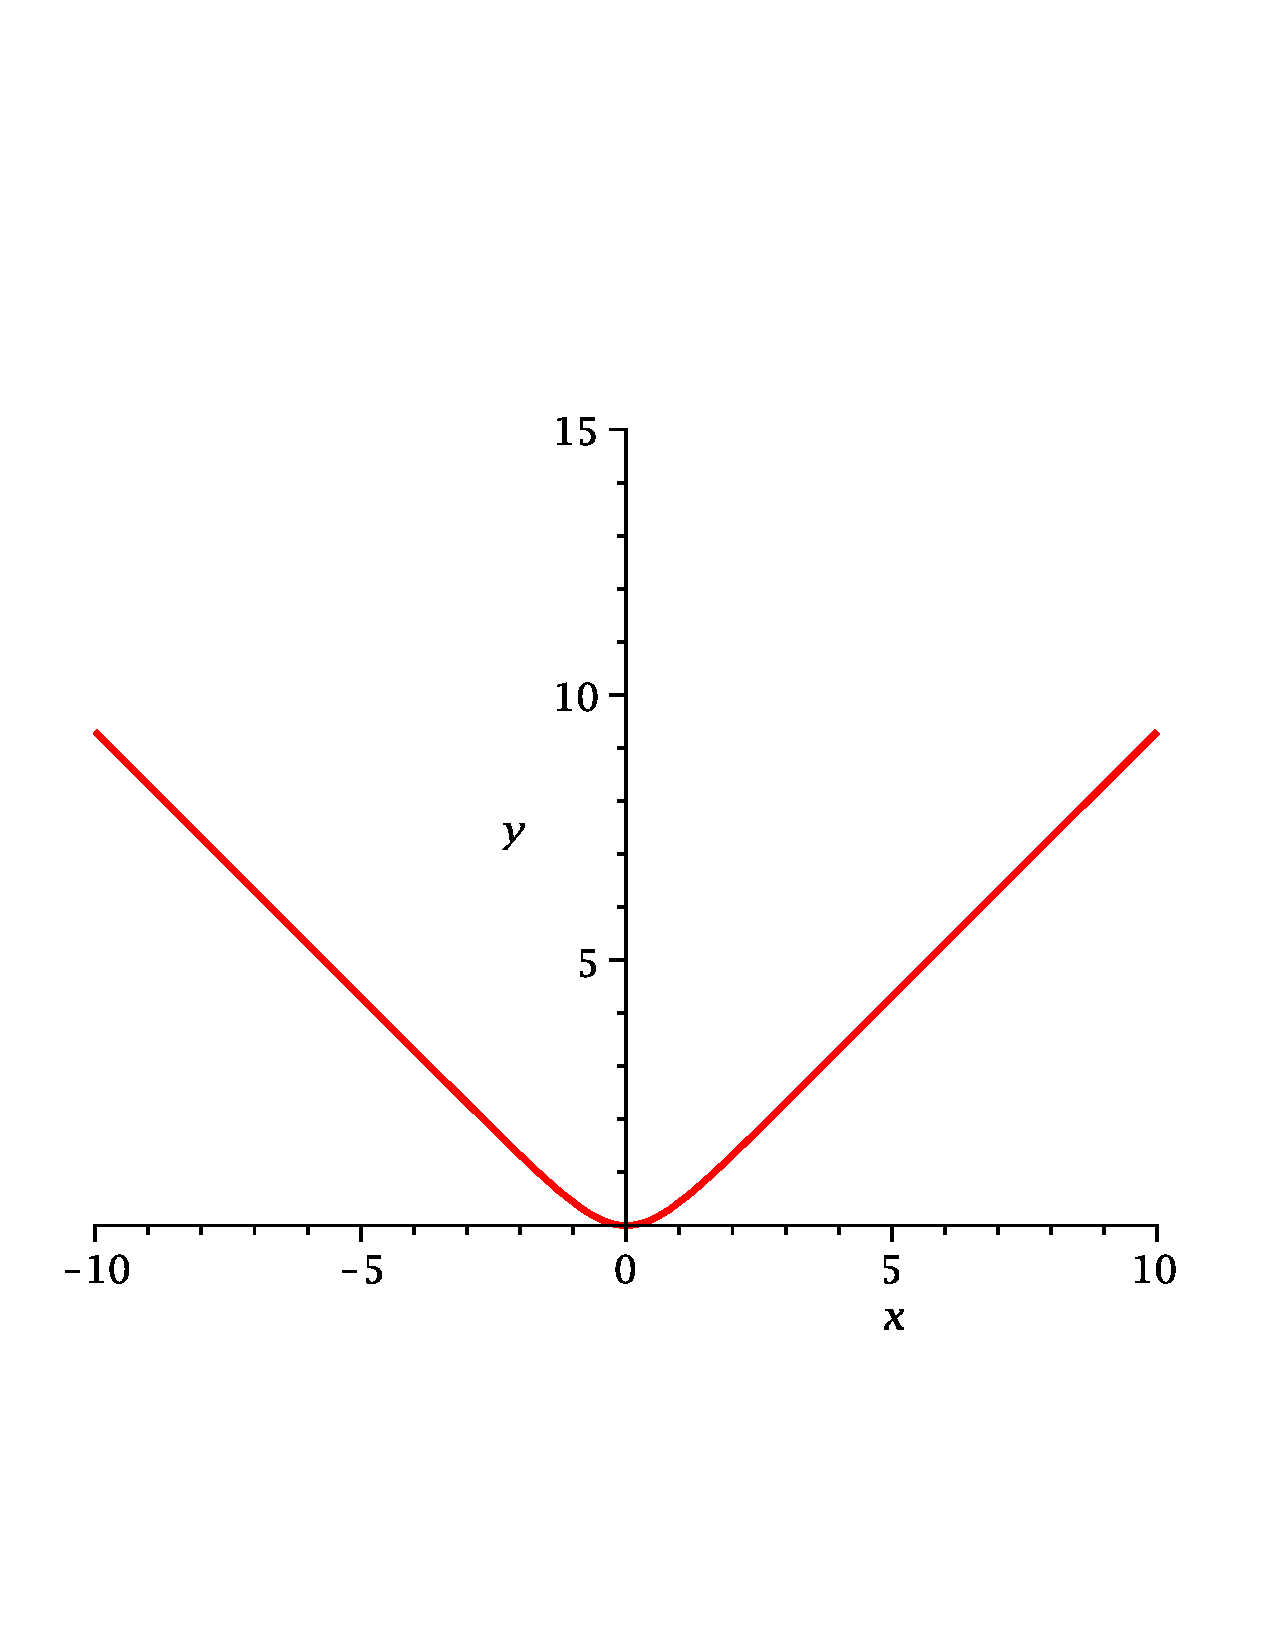
\includegraphics[scale=0.25]{Ecr01_7.pdf}
   \caption{Exercice \arabic{enumi} : courbe 7}
\end{figure}
Pour la recherche des points multiples de la deuxième ligne du tableau, on pourra montrer que si $t_1$ et $t_2$ sont les paramètres d'un (vrai) point multiple alors ils sont tous les deux congrus à $0$ ou a $\frac{\pi}{4}$ modulo $\frac{\pi}{6}$. Pour déterminer les points multiples former les tableaux des coordonnées pour ces valeurs du paramètre et chercher les doublons.  
 
  \item \begin{tiny}(Ecr02)\end{tiny}
\emph{Lemniscate.} Soit $S$ et $S^{\prime }$ les points de coordonn{\'e}es $(1,1)$ et $(-1,-1)$. Former l'{\'e}quation
cart{\'e}sienne de l'ensemble $\mathcal C_{k}$ des points $M$ tels que
\[
\left\| \overrightarrow{SM}\right\| \left\| \overrightarrow{S^{\prime }M}\right\| =k
\]
Pr{\'e}ciser $k_{0}$ pour que l'origine appartienne {\`a} $\mathcal C_{k_{0}}$. Trouver un param{\'e}trage rationnel de \emph{C}$_{k_{0}}$, tracer $\mathcal C_{k_{0}}$, former un param{\'e}trage polaire.
 
  \item \begin{tiny}(Ecr03)\end{tiny}
Préciser le support et étudier les questions particulières pour les paramétrisations polaires suivantes
\begin{align*}
 &r(t) = \cos(t) + \cos(2t)  \text{: points multiples}\\
 &r(t )=\sin \frac{2t }{3} \\
 &r(t )=1+\tan \frac{t }{2}  \text{ : point doubles, branches infinies}\\
 &r(t )=\frac{\ln (1+t)}{(1+t)^{2}}  \\
 &r(t)= \frac{1}{2\cos t\cos 2t}  \text{: branches infinies}\\
 &r(t )=\frac{1}{\sin t-\sin 2t} \text{: branches infinies}\\
 &r(t )=2\frac{\cos ^{2}t}{2\cos t-\sin t} \text{: branches infinies, pts stationnaires}\\
 &r(t)=\frac{1}{\sqrt{1+\sin 2t}+\sqrt{1-\sin 2t}}
\end{align*} 
  \item \begin{tiny}(Ecr04)\end{tiny}
La \emph{podaire} d'un point fix{\'e} par rapport {\`a} une courbe param{\'e}tr{\'e}e est la courbe form{\'e}e par la projection orthogonale de ce point sur les tangentes {\`a} la courbe.
\begin{figure}[ht]
 \centering
 \input{Ecr04_1.pdf_t}
 \caption{Exercice \arabic{enumi} : podaire d'un cercle.}
 \label{fig:Ecr04_1}
\end{figure}

\begin{enumerate}
\item Montrer que la podaire de l'origine par rapport {\`a} une spirale logarithmique $r(\theta )=ae^{m\theta }$ est une spirale semblable {\`a} la premi{\`e}re (c'est {\`a} dire image par une similitude)
\item Les \emph{lima\c{c}ons de Pascal} sont les podaires d'un cercle.\\
On considère un cercle de rayon $1$ et de centre le point de coordonnées $(-a,0)$ (figure \ref{fig:Ecr04_1}). On note $h(\theta)$ le projeté de l'origine du repère sur la tangente en $f(\theta)=0+\overrightarrow e_\theta$. Discuter suivant $a>0$ des variations de $x\circ h$ et du signe de $y\circ h$. Dessiner les diverses formes (en particulier la formation de la boucle) de lima\c{c}on. Dans le cas o{\`u} le point est sur le cercle, la courbe podaire est la \emph{cardio{\"\i}de}.
\end{enumerate} 
  \item \begin{tiny}(Ecr05)\end{tiny}
\emph{Propri{\'e}t{\'e}s de la cardio{\"\i}de}
La courbe est donn{\'e}e sous forme polaire par :
\[f(\theta)=O+(1+\cos \theta )\overrightarrow{e}_\theta\]
\begin{enumerate}
  \item Exprimer la direction de $\overrightarrow{f'}(\theta)$ en fonction de
  $\frac{3\theta}{2}$.
  \item Montrer que pour toute droite $\delta$ du plan, il
  existe trois points $M_1 , M_2 , M_3$ en lesquels la tangente est parall{\`e}le {\`a}
  $\delta$. Montrer que l'aire du triangle $(M_1 , M_2 , M_3)$ est
  constante.
  \item Soit $P$ et $Q$ deux points de la cardio{\"\i}de align{\'e}s avec
  O. Montrer que les tangentes sont orthogonales et que
  l'intersection de ces tangentes d{\'e}crit un cercle.
\end{enumerate} 
  \item \begin{tiny}(Ecr06)\end{tiny}
L' \emph{astro{\"\i}de} est la courbe
\[f(t)=(a\cos^3 t, a\sin^3 t)\]
Exprimer en polaire une courbe paramétrée telle que en chaque point de son support, on puisse mener deux tangentes orthogonales à l'astroïde. Dessiner les deux courbes. 
  \item \begin{tiny}(Ecr07)\end{tiny} Déterminer l'ensemble des cercles passant par $O$ et tangent à l'ellipse support de la courbe paramétrée $t\rightarrow O + 2\cos t \overrightarrow i + \sin t \overrightarrow j$. 
  \item \begin{tiny}(Ecr08)\end{tiny} Soit une courbe paramétrée (support noté $\mathcal C$)
\begin{displaymath}
 t\rightarrow M_t=O +t^2\overrightarrow i +t^3 \overrightarrow j
\end{displaymath} 
\'Ecrire l'équation de la tangente en $M_t$. Caractériser les points d'où on peut mener trois tangentes. Déterminer la courbe orthoptique de $\mathcal{C}$.  
  \item \begin{tiny}(Ecr09)\end{tiny} Une courbe de Lissajoux.\\
\'Etudier la courbe paramétrée
\begin{displaymath}
 t\rightarrow O + \cos t \overrightarrow i + \cos \frac{3t}{5}\overrightarrow j
\end{displaymath}
 Préciser en particulier l'intervalle d'étude, les points multiples et stationnaires. 
\end{enumerate} 
\clearpage 
\chead{courbes paramétrées: corrigés.}
\begin{enumerate}
  \item Les courbes paramétrées représentées par les figures de 1 à 7 sont respectivement celles de numéros : 2, 7, 1, 5, 3, 4, 6.
 
  \item Ccr02.tex manque. 
  \item Ccr03.tex manque. 
  \item Ccr04.tex manque. 
  \item Ccr05.tex manque. 
  \item Ccr06.tex manque. 
  \item \begin{tiny}(Ccr07)\end{tiny} Pour un point $\Omega_t$ de l'ellipse, on forme les équations de la normale en $\Omega_t$ à l'ellipse et de la médiatrice de $O\Omega_t$. Cela permet de calculer le point d'intersection et de former une paramétrisation de l'ensemble cherché. 
  \item L'équation de la tangente est $3tx+2y-5t^3=0$. Les points par où on peut mener trois tangentes sont ceux dont les coordonnées $x$, $y$ sont telles que la fonction $t \rightarrow 3tx+2y-5t^3$ s'annule trois fois. Formons le tableau de variations de cette fonction ... 
  \item Ccr09.tex manque. 
\end{enumerate} 
\end{document}